\documentclass[12pt]{article}
\usepackage{float}
\usepackage{harvard}
\usepackage[acronym]{glossaries}
\usepackage[automake]{glossaries-extra}
\usepackage{pgfgantt}
\usepackage{graphicx}
\usepackage{array}

\graphicspath{ {./images/} }


\makeglossaries

\newglossaryentry{ictal}
{
        name=latex,
        description={Is a mark up language specially suited for 
scientific documents}
}

\newglossaryentry{preictal}
{
        name=latex,
        description={Is a mark up language specially suited for 
scientific documents}
}

%\acrshort{gcd}
%\acrfull{gcd}
\newacronym{eeg}{EEG}{Electroencephalogram}
\newacronym{eegs}{EEGs}{Electroencephalograms}
\newacronym{ai}{AI}{Artificial Intelligence}
\newacronym{ml}{ML}{Machine Learning}
\newacronym{snr}{SNR}{Signal-to-Noise Ratio}
\newacronym{emd}{EMD}{Empirical Mode Decomposition}
\newacronym{svm}{SVM}{Support Vector Machine}
\newacronym{imf}{IMF}{Intrinsic Mode Functions}
\newacronym{csp}{CSP}{Common Spatial Pattern}
\newacronym{ga}{GA}{Genetic Algorithm}
\newacronym{loocv}{LOOCV}{Leaving One Out Cross-Validation}

\title{Project Proposal \\ Real-time preictal detection through the application of machine learning to Electroencephalogram signals.}
\author{William Riddell}

\begin{document}
\maketitle

\textit{Comments for Kashi will be written in italics. - William}

\section{Introduction}

Over the last 20 years, \acrfull{ai} has seen a large evolution through the use of \acrfull{ml}; the statistical analysis of data which leads to the unveiling of characteristics and connections. \cite{awad2015efficient}. There has been a large uptake of applying \acrshort{ml} techniques to biomedical data, increasing the speed and accuracy of prediction, detection, diagnosis, and prognosis. 

\acrfull{eegs} measure the electrical signals in the brain. \acrshort{eegs} have a great use in giving an insight into the inner workings of the brain, for example allowing us to pick up abnormalities preceding and during their occurrence. ``A seizure is a burst of uncontrolled electrical activity between brain cells (also called neurons or nerve cells) that causes temporary abnormalities in muscle tone or movements (stiffness, twitching or limpness), behaviours, sensations or states of awareness.'' \cite{johnHopkinsTypesOfSeizures} Due to this, monitoring the brain's electrical activity through the use of an \acrshort{eeg}, and applying analysis through an \acrshort{ml} model may allow us to detect the preictal period. ``An automated accurate prediction of seizures will significantly improve the quality of life of patients and reduce the burden on caregivers'' \cite{acharya2018automated}

This project will aim to develop an \acrshort{ml} model which triggers an alert if a preictal period is detected. The model will have to achieve a high degree of accuracy ($\geq90\%$) when being applied to real-time \acrshort{eeg} data. Throughout this project I will compare previous attempts using different \acrshort{ml} models, and I will evaluate the different datsets avaliable for preictal prediction. 


\section{Background Review}


\cite{wong2023eeg} reviews 10 datasets avaliable to download. It evaluates the way the EEGs were physically setup on the subject, the subjects themselves and the data's properties. Wong et al. also states their opinion on what tasks suite what dataset, with the main two tasks being either detection and prediction. 

\begin{table}[H]
\centering
\begin{tabular}{l}
\textbf{Dataset}                       \\
University of Bonn                   \\
CHB-MIT Scalp EEG                    \\
Melbourne-NeuroVista seizure trial (Neurovista Ictal)                           \\
Kaggle UPenn and Mayo Clinic's Seizure Detection Challenge                     \\
Neurology and Sleep Centre Hauz Khas \\
Kaggle American Epilepsy Society Seizure Prediction Challenge                  \\
Kaggle Melbourne-University AES-MathWorks-NIH Seizure Prediction Challenge \\
TUH EEG Seizure Corpus (TUSZ)        \\
Siena Scalp EEG                      \\
Helsinki University Hospital EEG    
\end{tabular}
\caption{10 Datasets within \protect\cite{wong2023eeg}}
\end{table}

Within these datasets Wong et al. was also able to find the way the EEG nodes were posistioned on the subject's cranium, along with whether the EEG nodes were either placed intracranial or extracranial. Wong et al. also the number of channels that are contained in the raw EEG data for each dataset.

\begin{table}[H]
\centering
\begin{tabular}{p{0.4\textwidth}p{0.1\textwidth}p{0.2\textwidth}p{0.2\textwidth}}
\textbf{Dataset}                                              & \textbf{Number of channels} & \textbf{Placement method}                & \textbf{Type of signal} \\
University of Bonn                                            & 1                           & International 10–20 system, Intracranial & Scalp/Intracranial EEG  \\
CHB-MIT Scalp EEG                                             & 18                          & International 10–20 system/Nomenclature  & Scalp EEG               \\
Melbourne-NeuroVista seizure trial (NeuroVista Ictal)         & 16                          & Intracranial                             & Intracranial EEG        \\
Kaggle UPenn and Mayo Clinic's Seizure Detection Challenge    & 16–76                       & Intracranial                             & Intracranial EEG        \\
Kaggle American Epilepsy Society Seizure Prediction Challenge & 16                          & Intracranial                             & Intracranial EEG        \\
Neurology and Sleep Centre Hauz Khas                          & 1                           & International 10–20 System               & Scalp EEG               \\
Kaggle Melbourne-University AES-MathWorks-NIH Seizure Prediction Challenge Data & 16 & Intracranial & Intracranial EEG \\
TUH EEG Seizure Corpus (TUSZ)                                 & 23–31                       & International 10–20 system / Nomenclature & Scalp EEG               \\
Helsinki University Hospital EEG                              & 19                          & International 10–20 system               & Scalp EEG               \\
Siena Scalp EEG                                               & 20/29                       & International 10–20 system/Nomenclature  & Scalp EEG              
\end{tabular}
\caption{\protect\cite{wong2023eeg}}
\end{table}

Wong et al. also noted along with this data that the ``University of Bonn dataset contains a mixture of both scalp and intracranial EEG data where scalp EEG from healthy subjects was taken, while intracranial EEG was taken from subjects with a history of seizures.'' \cite{wong2023eeg}. This may present a skew on the \acrshort{ml} model during training.


\begin{table}[H]
\centering
\begin{tabular}{p{0.4\textwidth}p{0.2\textwidth}p{0.2\textwidth}p{0.2\textwidth}}
  \textbf{Dataset} &
  \textbf{Noncontinuous data} &
  \textbf{Short-term continuous data} &
  \textbf{Continuous data} \\
  
University of Bonn                                                              & Yes & No  & No  \\
CHB-MIT Scalp EEG                                                               & No  & Yes & Yes \\
Melbourne-NeuroVista seizure trial (Neurovista Ictal)                           & N/A & N/A & N/A \\
Kaggle UPenn and Mayo Clinic's Seizure Detection Challenge                      & Yes & No  & No  \\
Kaggle American Epilepsy Society Seizure Prediction Challenge                   & Yes & No  & No  \\
Neurology and Sleep Centre Hauz Khas                                            & Yes & No  & No  \\
Kaggle Melbourne-University AES-MathWorks-NIH Seizure Prediction Challenge Data & Yes & No  & No  \\
TUH EEG Seizure Corpus (TUSZ)                                                   & No  & Yes & No  \\
Helsinki University Hospital EEG                                                & No  & Yes & No  \\
Siena Scalp EEG                                                                 & No  & Yes & No 
\end{tabular}
\caption{\protect\cite{wong2023eeg}}
\end{table}

Wong et al. ordered the datasets into groups, either continuous or non continuous data. For the continuous data they seperated out datasets which record for less that 24 hours in a single go, these were classified as ``Short-term continuous'' data.

%TODO add more tables from the wong2023eeg dataset


Dataset CHB-MIT \cite{shoeb2009application} \cite{PhysioNet} was taken from Boston Children's Hospital. It is a long-term dataset with recordings of 22 paediatric subjects, 5 male and 17 female, who have intractable seizures. The dataset contains 23 \acrshort{eeg} signals positioned on the scalp in the international 10-20 \acrshort{eeg} system \cite{sharbrough1991american}. The dataset is labelled with the timestamps of the onset and ending of each seizure. Over the course of several days the onsets and ends of a total of 182 seizures were annotated onto the long-term EEG data \cite{shoeb2009application} \cite{PhysioNet}. This dataset is utilized by many papers when working on real-time epileptic seizure detection, there have been many different approaches with detection accuracy reaching 92.23\% \cite{usman2017epileptic}


Usman et al. was able to achieve a preictal detection rate (sensitivity) of 92.23\% against the CHB-MIT dataset. \cite{usman2017epileptic} Usman noted that poor \acrfull{snr} within the dataset lead to a large amount of false positives and posed as a issue during his research. To combat this he combined the many \acrshort{eeg} signals into a single surrogate signal and then utilized \acrfull{emd} to increase the \acrshort{snr}. Usman et al. then broke the surrogate signal down and ``extracted multiple features including entropy, approximate entropy, and Hjorth parameters.'' In Usman's et al. papers, it was observed that both statistical and spectral features played a part in detecting the differences between interictal and preictal states so he also extracted spectral moments, and statistical moments to aid with his classification. He finally utilized a \acrfull{svm} taking in a continuous \acrshort{eeg} signal broken into non-overlapping one second sections and classifying if it was part of a preictal period \cite{usman2017epileptic}.


Gao at al. also used the CHB-MIT dataset to train various \acrshort{ml} models, although they developed a system which assigns weights to each sample in the dataset, and then uses a \acrfull{ga} to optimize the weights according to the increase of accuracy of prediction when applied to their validation set \cite{gao2022general}. Gao's et al. approach solved some common issues that surface when attempting to predict preictal periods; \acrshort{eeg} signals when monitoring epileptic seizures face an class imbalance problem, to address this researchers normally reduce the number of interictal samples \cite{ozcan2019seizure}, or increase the number of preictal periods, often using generative methods \cite{usman2021deep}, but as Gao et al. stated, this increased the uncertainty in the model. Goa et al. approach of assigning weights to samples avoids this downfall. Another benefit of applying Gao at al. methodology is the avoidance of the noisy label problem. This is where there is no standardized preictal period, with most researchers applying their own empirical fixed time length before the seizure. This can vary from 2 minutes before the ictal period to 30 minutes. By applying weights to different samples the \acrshort{ml} model ``can select and focus on more valuable samples for seizure prediction. These samples prompt the model to perform better on the validation set, thus further improving the generalization of the model.'' \cite{gao2022general}. Gao et al. was able to achieve a sensitivity of 85.9\%, and a false positive rate / hour of 0.09. 


Other methods for predicting seizures exist, although they are outside the realm of \acrshort{ml}. When a seizure occurs, or during the preictal state, the spike rate and variation in the \acrshort{eeg} signals change \cite{lange1983temporo} \cite{truccolo2011single} ``spike rate is used as the indicator to anticipate seizures in \acrfull{eeg} signal. Spikes detection step is used in \acrshort{eeg} signal during interictal, preictal, and ictal periods followed by a mean filter to smooth the spike number. The maximum spike rate in interictal periods is used as an indicator to predict seizures.'' \cite{slimen2020epileptic}. Using this method, Slimen et al. was able to achieve a 92\% accuracy. \textit{This is an interesting approach, although not ML, I wonder if I can use it to aid in my ML methodology?}


\section{Methodology}

\subsection{Approach (Description of the research and development methodology, e.g. Software
development model, requirement gathering method, test and evaluation process)}

I will be utilizing the open-source CHB-MIT dataset \cite{shoeb2009application} \cite{PhysioNet} as it contains all ictal periods which is ideal for the prediction of epileptic seizures. I will be following the preprocessing stages that Usman et al. and Gao et al used. This involves converting the \acrshort{eeg} signals into a single signal through the use of applying an averaging filter and the \acrfull{csp} algorithm to increase the \acrshort{snr}. Once I have applied these algorithms I will perform \acrshort{emd} which breaks the surrogate signal into its oscillatory functions, which are amplitude, period, and frequency. This is also known as its \acrfull{imf}. I will also be applying the sample weighting methodology used in \cite{gao2022general} to aid in my prediction.

\begin{table}[H]
\centering
\begin{tabular}{lllll}
                             & \textbf{Features}    &  &  &  \\
\textbf{Statistical moment}  & Mean                 &  &  &  \\
                             & Variance             &  &  &  \\
                             & Skewness             &  &  &  \\
                             & Kurtosis             &  &  &  \\
\textbf{Spectral band power} & Delta (0.5 – 4 Hz)   &  &  &  \\
                             & Theta (4–8 Hz)       &  &  &  \\
                             & Alpha (8–13 Hz)      &  &  &  \\
                             & Beta (13–30 Hz)      &  &  &  \\
                             & Gamma-1 (30–50 Hz)   &  &  &  \\
                             & Gamma-2 (50–75 Hz)   &  &  &  \\
                             & Gamma-3 (75–100 Hz)  &  &  &  \\
                             & Gamma-4 (100–128 Hz) &  &  &  \\
\textbf{Hjorth parameters}   & Mobility             &  &  &  \\
                             & Complexity           &  &  & 
\end{tabular}
\caption{Proposed Features to extract}
\end{table}

I will be programming the preprocessing and the ML model in Python 3 \cite{python3}, using library's such as TensorFlow \cite{tensorflow2015-whitepaper} which I will be using to construct my \acrshort{svm}. I will also be using Numpy \cite{harris2020array} to write in my averaging filter and \acrshort{csp} algorithm. I will also be using the ``EMD-signal'' library \cite{pyemd} to split the surrogate signal into its \acrshort{imf}. Using the \acrfull{loocv} methodology I will be fine tuning the \acrshort{ml} model against different sample weights as stated in \cite{gao2022general}. 

I will be version managing this project using the software ``Git'' , and hosting the repository on ``Github'', and I will be using my own hardware, a Nvidia GeForce GTX 1080, to train the \acrshort{svm}. For testing purposes I will be using the libraray PyTest to unit test my functions, and as mentioned above I will be using \acrshort{loocv} to test my \acrshort{ml} model.

\section{Project management}
\subsection{Activities}

\begin{enumerate}
    \item Data Collection and Preprocessing:
    \begin{itemize}
        \item Download the CHB-MIT dataset.
        \item Preprocess EEG signals:
        \begin{itemize}
            \item Apply averaging filter to combine EEG signals.
            \item Implement Common Spatial Pattern (CSP) algorithm for noise reduction.
            \item Perform Empirical Mode Decomposition (EMD) to extract Intrinsic Mode Functions (IMF).
        \end{itemize}
    \end{itemize}
    
    \item Feature Extraction:
    \begin{itemize}
        \item Extract features. See Table 1.
        \item Apply the sample weighting methodology used in \cite{gao2022general} for feature weighting.
    \end{itemize}
    
    \item Model Development:
    \begin{itemize}
        \item Train a Support Vector Machine (SVM) using the preprocessed features.
        \item Tune SVM hyper-parameters for optimal performance using \acrshort{loocv}.
    \end{itemize}
    
    \item Testing and Evaluation:
    \begin{itemize}
        \item Evaluate the SVM model using performance metrics.
        \item Validate the prediction accuracy and sensitivity with a test dataset.
    \end{itemize}
    
    \item Documentation:
    \begin{itemize}
        \item Maintain project logs, reports, and literature references within the Git repository.
        \item Document the entire process throughout the development.
    \end{itemize}
    
    \item Project Reporting:
    \begin{itemize}
        \item Create a final project report summarizing the methodology, results, and conclusions.
        \item Implement any additional information, such as documentation and sources.
    \end{itemize}
\end{enumerate}


\subsection{Schedule}

\begin{figure}[H]
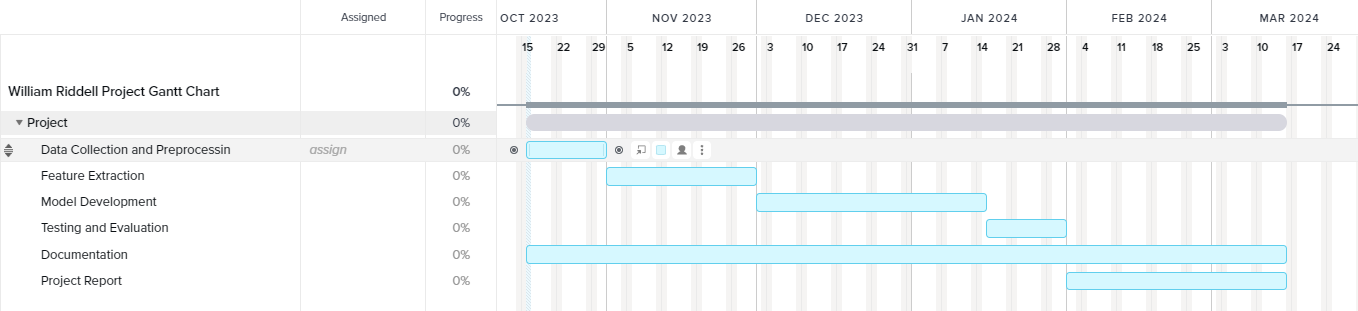
\includegraphics[width=\textwidth]{gantt}
\centering
\end{figure}


\subsection{Deliverables}

\begin{itemize}
    \item A well-documented real-time epileptic seizure prediction model using EEG signals from the CHB-MIT dataset.
    \item A final project report outlining the methodology, results, and conclusions.
    \item Included in the project report, logs documenting activities, tasks, and changes throughout the project.
    \item Organized data, including raw data, the preprocessed data, and relevant literature.
\end{itemize}



\pagebreak

\printglossary[type=\acronymtype]
\printglossary

\pagebreak

\bibliographystyle{agsm}
\bibliography{references}

\end{document}